\documentclass[12pt, a4paper, oneside]{article}
\usepackage{arial}
\renewcommand{\familydefault}{\sfdefault}
\usepackage[T1]{fontenc}
\usepackage[polish]{babel}
\usepackage[utf8]{inputenc}
\usepackage{lmodern}
\usepackage[left=2cm,right=2cm,top=2cm,bottom=2cm]{geometry}
\selectlanguage{polish}
\usepackage{graphicx}
\usepackage{longtable}

\begin{document}
\section{Wykorzystane wzory}
Niepewność zmierzonej długości linii
\begin{equation}
u(L)=\frac{\Delta_{siatki}}{\sqrt{3}}
\end{equation}
Powiększenie interferometru
\begin{equation}
k=\frac{L_1}{L_0}
\end{equation}
Niepewność wyznaczonego powiększenia interferometru
\begin{equation}
u_C(k)=\sqrt{(\frac{\partial k}{\partial L_0})^2\cdot u^2(L_0)+(\frac{\partial k}{\partial L_1})^2\cdot u^2(L_1)}=\sqrt{\frac{L_1^2}{L_0^4}\cdot u^2(L_0)+\frac{1}{L_0^2}\cdot u^2(L_1)}
\end{equation}
Kąt nachylenia klina (próbka nr 2)
\begin{equation}
\phi=\frac{\lambda}{2}\cdot\frac{\Delta K_{AB}}{l_{AB}}
\end{equation}
Niepewność wyznaczonego kąta nachylenia klina (próbka nr 2)
\begin{equation}
u_C(\phi)=\sqrt{(\frac{\partial\phi}{\partial l_{AB}})^2\cdot u^2(l_{AB})}=\frac{\lambda}{2}\cdot\frac{\Delta K_{AB}}{l^2_{AB}}\cdot u(l_{AB})
\end{equation}
Promień krzywizny powierzchni sferycznej (próbka nr 3)
\begin{equation}
R=\frac{d_K^2}{4\cdot\lambda\cdot K}
\end{equation}
Niepewność wyznaczonego promienia powierzchni sferycznej (próbka nr 3)
\begin{equation}
u_C(R)=\sqrt{(\frac{\partial R}{\partial d_K})^2\cdot u^2(d_K)}=\frac{d_K}{2\cdot\lambda\cdot K}\cdot u(d_K)
\end{equation}
\section{Przykładowe obliczenia}
Niepewność zmierzonej długości linii
\begin{center}
$u(L)=\frac{0.1}{1.73}=0.058~[cm]$
\end{center}
Powiększenie interferometru
\begin{center}
$k=\frac{1.2}{1}=1.200$
\end{center}
Niepewność wyznaczonego powiększenia interferometru
\begin{center}
$u_C(k)=\sqrt{\frac{(1.2)^2}{1^4}\cdot(0.58)^2+\frac{1}{1^2}\cdot(0.58)^2}=0.091$
\end{center}
Kąt nachylenia klina (próbka nr 2)
\begin{center}
$\phi=\frac{589.3 \cdot 10^{-9}}{2}\cdot\frac{5}{6.72 \cdot 10^{-3}}=219.32 \cdot 10^{-6}~[rad]$
\end{center}
Niepewność wyznaczonego kąta nachylenia klina (próbka nr 2)
\begin{center}
$\phi=\frac{589.3 \cdot 10^{-9}}{2}\cdot\frac{5}{(6.72 \cdot 10^{-3})^2}\cdot 0.58\cdot10^{-3}=0.019\cdot 10^{-6}~[rad]$
\end{center}
Promień krzywizny powierzchni sferycznej (próbka nr 3)
\begin{center}
$R=\frac{(3.44\cdot10^{-2})^2}{4\cdot589.3\cdot10^{-9}\cdot10}=50~[m]$
\end{center}
Niepewność wyznaczonego promienia powierzchni sferycznej (próbka nr 3)
\begin{center}
$u_C(R)=\frac{3.44\cdot10^{-2}}{2\cdot589.3\cdot10^{-9}\cdot10}\cdot 0.58=17~[m]$
\end{center}
\clearpage
\section{Wyniki pomiarów i opracowanie}
\begin{figure}[h]
\centering
\caption{Odrysowana linia odniesienia pozwalająca określić powiększenie interferometru}
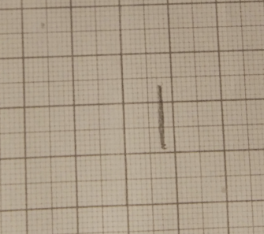
\includegraphics[scale=.8]{pics/f1.png}
\end{figure}
\begin{figure}[h]
\centering
\caption{Prążki interferencyjne - próbka numer 1}
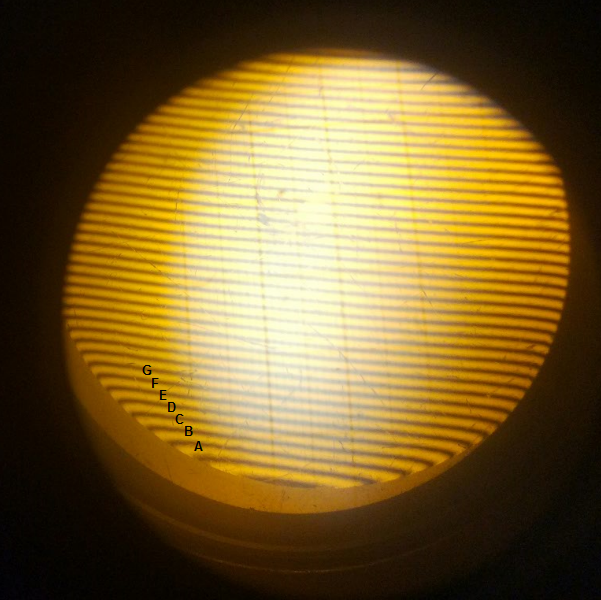
\includegraphics[scale=.6]{pics/f2.png}
\end{figure}
\clearpage
\begin{figure}[t]
\centering
\caption{Prążki interferencyjne - próbka numer 2}
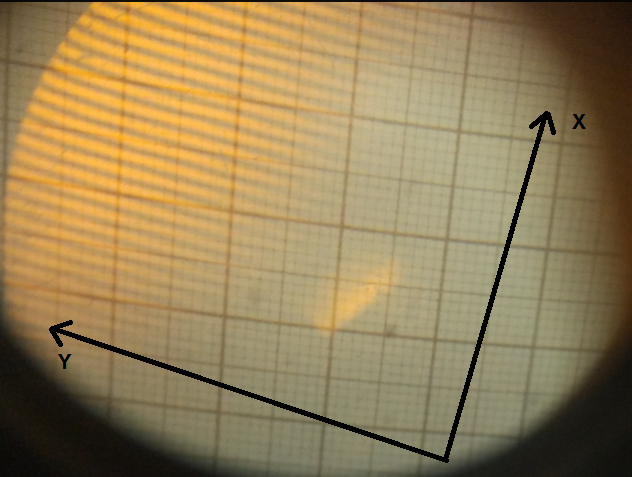
\includegraphics[scale=.55]{pics/f2_1.png}
\end{figure}
\begin{figure}[b]
\centering
\caption{Model nachylenia próbki numer 2 (rys. 3)}
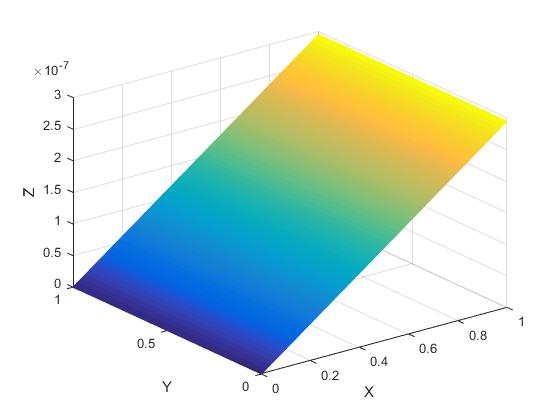
\includegraphics[scale=0.55]{pics/w1.jpg}
\end{figure}
\begin{figure}[t]
\centering
\caption{Prążki interferencyjne (pierścienie Newtona) - próbka numer 3}
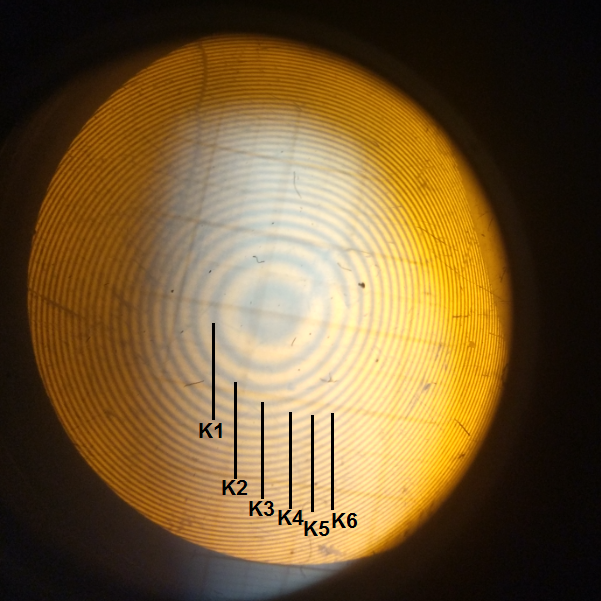
\includegraphics[scale=.55]{pics/f4.png}
\end{figure}
\begin{figure}[b]
\centering
\caption{Model próbki numer 3 (rys. 5)}
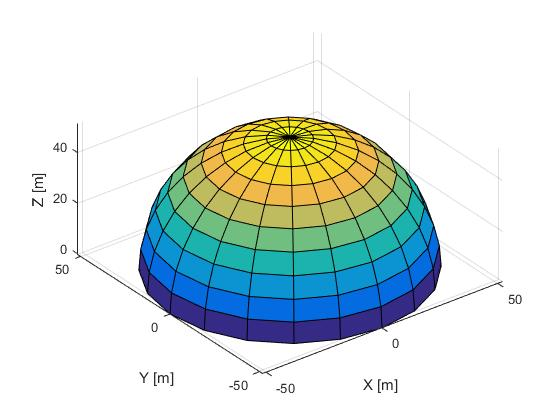
\includegraphics[scale=.55]{pics/w2.jpg}
\end{figure}
\clearpage
\begin{figure}[t]
\centering
\caption{Prążki interferencyjne - próbka numer 4}
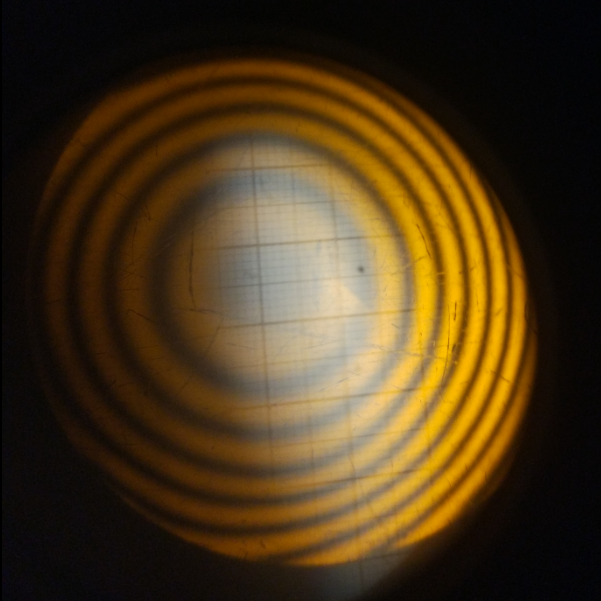
\includegraphics[scale=.4129]{pics/f5.png}
\end{figure}
\begin{figure}[b]
\centering
\caption{Prążki interferencyjne - próbka numer 5}
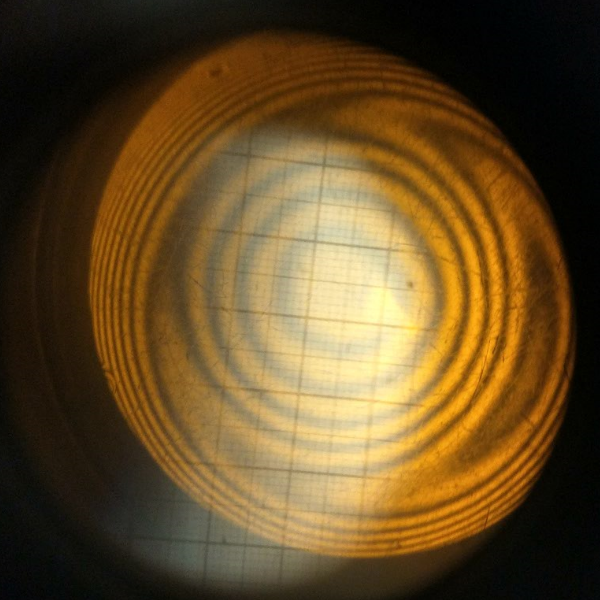
\includegraphics[scale=.4129]{pics/f6.png}
\end{figure}
\clearpage
\begin{figure}[t]
\centering
\caption{Prążki interferencyjne - próbka numer 6}
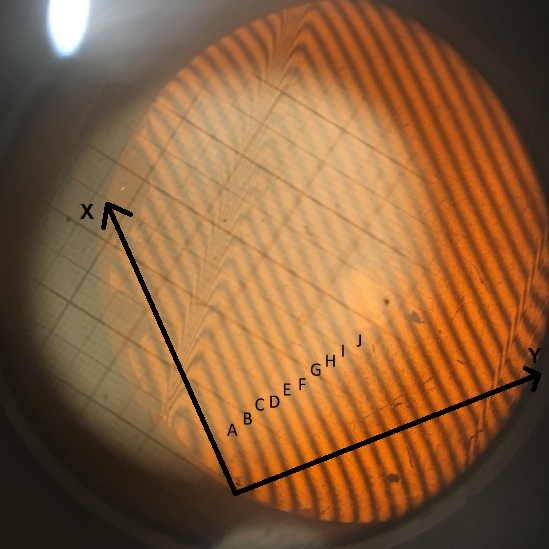
\includegraphics[scale=.4129]{pics/f7.png}
\end{figure}
\clearpage
% Table generated by Excel2LaTeX from sheet 'Arkusz1'
\begin{table}[h]
  \centering
  \caption{Wyniki pomiarów dla próbki nr 2 (rys. 3)}
    \begin{tabular}{|c|c|c|c|c|}\hline
    $\Delta K_{AB}$ & $l_{AB}~[mm]$ & $u(l_{AB})~[mm]$ & $\phi\cdot 10^{-6}~[rad]$ & $u_C(\phi)\cdot 10^{-6}~[rad]$ \\\hline
    1 & 1.33 & 0.58 & 221.9 & 0.1 \\\hline
    2 & 2.72 & 0.58 & 216.862 & 0.047 \\\hline
    3 & 4.03 & 0.58 & 219.299 & 0.032 \\\hline
    4 & 5.40 & 0.58 & 218.281 & 0.024 \\\hline
    5 & 6.72 & 0.58 & 219.319 & 0.019 \\\hline
    6 & 8.09 & 0.58 & 218.562 & 0.016 \\\hline
    7 & 9.37 & 0.58 & 220.112 & 0.014 \\\hline
    8 & 10.66 & 0.58 & 221.175 & 0.013 \\\hline
    9 & 12.02 & 0.58 & 220.704 & 0.011 \\\hline
    10 & 13.54 & 0.58 & 217.5877 & 0.0094 \\\hline
    15 & 20.50 & 0.58 & 215.6261 & 0.0062 \\\hline
    \multicolumn{5}{|c|}{Wartość średnia kąta nachylenia klina} \\\hline
    \multicolumn{5}{|c|}{$\phi$ = (219.038 $\pm$ 0.012) $\cdot$ 10$^{-6}$ rad} \\\hline
    \end{tabular}%
  \label{tab:addlabel}%
\end{table}%
% Table generated by Excel2LaTeX from sheet 'Arkusz1'
\begin{table}[h]
  \centering
  \caption{Wyniki pomiarów dla próbki nr 3 (rys. 4)}
    \begin{tabular}{|c|c|c|c|c|}\hline
    $K$ & $d_K~[cm]$ & $u(d_K)~[cm]$ & $R~[m]$ & $u_C(R) ~[m]$ \\\hline
    1 & 1.21 & 0.58 & 62 & 60 \\\hline
    2 & 1.64 & 0.58 & 57 & 41 \\\hline
    3 & 1.97 & 0.58 & 55 & 33 \\\hline
    4 & 2.26 & 0.58 & 54 & 28 \\\hline
    5 & 2.51 & 0.58 & 53 & 25 \\\hline
    6 & 2.72 & 0.58 & 52 & 23 \\\hline
    7 & 2.93 & 0.58 & 52 & 21 \\\hline
    8 & 3.12 & 0.58 & 52 & 20 \\\hline
    9 & 3.29 & 0.58 & 51 & 18 \\\hline
    10 & 3.44 & 0.58 & 50 & 17 \\\hline
    11 & 3.59 & 0.58 & 50 & 17 \\\hline
    \multicolumn{5}{|c|}{Wartość średnia promienia krzywizny} \\\hline
    \multicolumn{5}{|c|}{(K$_1$, K$_2$ i K$_3$ zostały pominięte)} \\\hline
    \multicolumn{5}{|c|}{R = (51.8 $\pm$ 7.5) [m]} \\\hline
    \end{tabular}%
  \label{tab:addlabel}%
\end{table}%

\section{Wnioski}
\begin{itemize}
\item Powiększenie optyczne przyrządu wynosi k = 1.2 $\pm$ 0.091.
\item Kąt nachylenia klina (próbka numer 2) wynosi $\phi$ = (219.038 $\pm$ 0.012) $\cdot$ 10$^{-6}$ rad.
\item Kąt $\phi$ zaobserwowany podczas zajęć był praktycznie niewidoczny, co może odpowiadać wyznaczonej wartości.
\item Promień powierzchni sferycznej (próbka numer 3) wynosi R = (51.8 $\pm$ 7.5) [m] i~jest to powierzchnia wypukła.

\end{itemize}
\end{document}